\documentclass[Japanese]{dicomopapers}
%\documentclass[Japanese,noauthor]{dicomopapers}

\usepackage[dvipdfmx]{graphicx}
\usepackage{latexsym}
\usepackage{otf}
\usepackage[hyphens]{url}
\usepackage{comment}

\def\Underline{\setbox0\hbox\bgroup\let\\\endUnderline}
\def\endUnderline{\vphantom{y}\egroup\smash{\underline{\box0}}\\}
\def\|{\verb|}

% %概要投稿用余白調整ここから
% \setlength{\Jauthorjreceivesep}{0.0mm}
% \setlength{\Jreceivejabstsep}{0.0mm}
% \setlength{\Jabstsepjkeyword}{0.0mm}
% \setlength{\Jkeywordetitle}{0.0mm}
% %概要投稿用余白調整ここまで

\begin{document}

% 和文表題
\title{異種無線による電力効率化のための\\ノードのグループ構成手法のシミュレーション}
% 英文表題
\etitle{Simulation of Node Group Construction Method for Energy Efficiency}
% 所属ラベルの定義
\affiliate{FUN1}{公立はこだて未来大学大学院 システム情報科学研究科}
\affiliate{FUN2}{公立はこだて未来大学 システム情報科学部}
% 著者
\author{戸澤 涼}{RYO TOZAWA}{FUN1}
\author{稲村 浩}{HIROSHI INAMURA}{FUN2}
\author{中村 嘉隆}{YOSHITAKA NAKAMURA}{FUN2}
% 概要
\begin{abstract}
IoT センサデバイスは,バッテリー駆動が前提となるため省電力化が重要である.LoRaWAN は,無線センサネットワーク(WSN:Wireless Sensor Network)において省電力で広域カバレッジを実現している.LoRaWAN には,WSN 内のデバイス増加時にメッセージ衝突によるパケット到達率低下というスケーラビリティでの課題がある.本研究では,WSN内で複数ノードのグループを自律的に構成し代表がデータを集約し代理送信する手法を基本に遠距離,近距離において異種通信を使い分けることで,WSN の電力効率化を図る.先行研究として,異種無線を組み合わせた場合と既存のLoRaのみのWSNにおける消費電力の差異を実測にて検証し,提案したプロトコルを用いた際のデータの集約による消費電力の効率化に関する消費電力のモデル式を実測データで評価により提案手法の有効性を提示した.本稿では,提案手法の有効性を評価するために応用として,実環境においてゴミ収集のIoT化を推進した場合,提案手法を用いた場合の方がLoRaWANのみの既存ソリューションと比較し,消費電力の観点で有効であるかをネットワークシミュレーターのns3を用いて評価する.
\end{abstract}

% 表題などの出力
\maketitle

% 本文はここから始まる
% 問題と貢献
\section{はじめに}
WSN(WSN: Wireless Sensor Network)は,IoTにおけるセンサネットワーク技術である.IoTの利用用途は,環境モニタリング,ビル管理,スマートホーム等が挙げられる.IoTの代表例となるセンサデバイスは,バッテリ駆動の制約によるデバイスの省電力化及び遠隔におけるノード管理の必要性,低伝送量,ノード数の増加によるネットワークの混雑等が課題となっている.これらの課題に対し,WSNにおいて省電力で広域カバレッジを特徴とする省電力広域通信規格の一つであるLoRaWANが選択肢として注目されている.LoRaWANとは,LoRaという長距離通信を特徴とした省電力広域ネットワークプロトコルである.スター型のトポロジや免許不要の周波帯を利用しているためネットワーク構築が低コストで可能であることが可能である.しかし,LoRaWANの課題として,ネットワーク内のデバイス数が増加した際にパケット到達率が低下するという課題がある.以上の背景から,LoRaWANについて,スケーラビリティを考慮した高集積なセンサネットワークの研究が行われている.既存手法では,WSN内で幾つかのセンサからなるグループを作成しグループの代表がセンサ情報を集約し代理送信することで,ネットワークの収容数向上と消費電力量削減の可能性を提示した.しかし,グループ構成手法を用いるには,センサ間の直接通信が必要になる.LoRaWANのみでは仕様上実現が困難である上に,グループの生成や維持などにおける具体化が求められる.そこで我々は先行研究として,消費電力(削減・平準化)の観点で,市販されているLoRaWANとBLEが搭載されたモジュールに着目し,遠距離通信はLoRaWAN,近距離通信はBLEを用いることで異種通信の消費電力を考慮したグループ構成手法を提案し,電力実測実験のもと有効性を提示した.

\par
本稿では,提案手法の有効性を評価するために応用として,実環境においてゴミ収集のIoT化を推進した場合,提案手法を用いた場合の方がLoRaWANのみの既存ソリューションと比較し,消費電力の観点で有効であるかをネットワークシミュレーターのns3を用いて評価する.

\section{関連研究}
\subsection{LoRaWANにおけるネットワーク効率化のためのノードのグループ化構成法と通信制御方式}
LoRaWANにはノード数のスケーラビリティ,及び拡散率による通信時間が大きく異なるという課題がある.手柴らが提案する手法\cite{group}は,消費電力量を抑制しセンサノードのバッテリ寿命を延伸するため,GWとセンサノードの距離,ノード数,消費電力量をもとにノードのグループを作成し,GC(GC: Group Coordinator)と呼ぶセンサノードを経由して通信する.想定環境は,ノードが均一に分布されたネットワークであり,センサノードが持つ通信モジュールはスケジュールされた時刻に下り受信が可能なLoRaWAN のクラスBである.アプローチを下記に示す.センサノードはネットワークに参加後,指定されたグループ内のGCを経由しデータを送信する.通信時間による消費電力量効率化のため,拡散率とそれに伴う通信時間をもとに,同一周波数を異なる時間のスロットへ分割する.グループの構成により,センサノード全てがGWと接続する既存モデルと比較し合計送信時間が削減される可能性がある.拡散率を考慮した時間スロットの割当により,同一周波数を一定時間で分割する時分割多元接続(TDMA: Time Division Multiple Access)により時間スロットの効率的な割当が可能となると述べている.
\par
課題として,グループ化にはセンサノード間での通信が必要となるが,LoRaWAN の仕様上,実現が困難である点,グループ編成時にネットワークサーバにセンサノードの物理的位置を手動で登録しなければならない点つまり動的なノードの変化への対応が困難であることやGCにLoRaWANの利用が集中することによる消費電力増加が考慮されていない点等があげられる.そこで本研究では,グループ化手法を活かし異種無線を用いた消費電力効率化,及びノードの情報を用いて自律的にグルーピングを行う.

\subsection{LPWA通信を利用するIoTプラットフォーム向けの電力効率を考慮したゲートウェイ配置手法の検討}
辻丸らが提案する手法\cite{gateway}は,センサノードの消費電力を平準化するため,LoRaWANにおけるゲートウェイの配置を最適化するものである.LoRaWANのようなスター型トポロジの無線ネットワーク構成であると,ノード間の通信距離と消費エネルギーの差異を考慮する必要がある.本研究では,LoRaWANにおける拡散係数を考慮することで通信距離と消費エネルギーのトレードオフを考慮しゲートウェイを複数配置し輻輳を減少させ消費電力を削減している.
\par
課題として,拡散率をエネルギー消費のみでノードに割り当てているため,同様の拡散率が割り当てられたセンサノードが密集した場合の衝突可能性が考慮されていない点,ゲートウェイの同時接続数の上限が考慮されていないため,通信の衝突可能性が考慮されていない点が挙げられる.本システムでは既存の
LoRaWANが提供する機能を用いて解決する.

\section{提案方式}
提案方式では,LoRaWANネットワークにおいて電力効率化のためのグループ化方式の実現を目的とする.
ここで,電力効率化とはノードの消費電力削減及び各ノードの消費電力量が均一となる平準化を含む.

\subsection{グループ化}
異種無線によるグループ化の具体的な手法とプロトコルを示す.

\subsubsection{センサノード間通信}
LoRaWANの長距離伝送の回数を減らし,センサネットワーク全体の消費電力削減するため,異種無線(LoRaWAN, BLE)(図\ref{group_topology}参照)を適用する.集約ノード(GL: Group Leader)は,グループ内はBLE,ゲートウェイとはLoRaWANを用いてデータの送受信を行う.通常ノード(GM: Group Member)は,BLEにてデータの送受信を行う.

\begin{figure}[h]
    \centering
    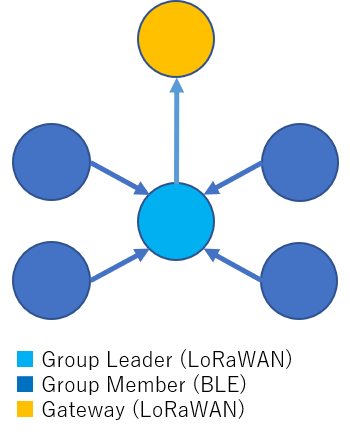
\includegraphics[width=5cm]{./img/group_topology.png}
    \caption{グループ化のトポロジ}
    \label{group_topology}
\end{figure}

\subsubsection{グループ構成法}
既存手法\cite{group}ではグループを作成する際に,全てのセンサノードの位置を事前にLoRaWANのNSが把握していることが前提条件となっている.ネットワーク運用者の管理コストを削減するため,センサ起動時に周囲のセンサノード情報を取得しNSに提供することで,センサノード増減に合わせ能動的にグループを構成する.
\par
センサ起動からグループを作成するまでのプロトコルを説明する.センサは起動時に,データ収集時間($T_{da}$: Data Acquisition Time)の間,BLEを用いて(表参照)を発信するとともに,(表参照)を受信する.起動から$T_{da}$経ったのち,NSへ送信する.その際,NSには以下の情報(表参照)が集まる.NSは,重複を排除したのち,お互いに到達可能なノード同士でグループを作成し,各ノードからみた信号強度が最も高いノードをGLとする.

\subsubsection{電力平準化のためのグループ再構成}
既存手法\cite{group}では,GCがグループ内のセンサノードの通信を集約すると述べていた.これにより,GWに接続するセンサノードが減りスケーラビリティを向上させることができる.しかし,GCでの通信回数が増加するため,GCの消費電力量の増加が顕著になることが懸念される.消費電力平準化のため,バッテリ残量を推測しグループ内におけるGLの入れ替えを行う.
\par
グループ再構成のプロトコルを説明する.各ノードは,異種無線の通信回数をローカルに保持し,GLがその値を元に各センサのバッテリ残量を推測する.そして,バッテリ残量に余裕のあるノードを次のGLとしグループに通知する.
    
\subsubsection{センサノードの近接性を考慮した拡散率・通信タイミング割当の検討}
既存研究\cite{gateway}では,LoRaWANは長距離通信になるほど消費電力が増加するため,GWノードとセンサノードの距離をもとに適切な拡散率を割り当てていた.しかし,シミュレーションの環境が密集した住宅街であったため,隣接したノードが同様の拡散率のもと通信を開始した場合に,衝突が発生し,パケット到達率が大きく低下することが懸念される.グループ化にも同様のことが言え,隣接したグループにおいて,拡散率の割当や通信タイミングの制御を検討する必要がある.提案方式では,拡散率の割当は,GWとの距離により適切な拡散率を割り当てるLoRaWANのADR(ADR: Adaptive Data Rate)機能を用い,通信タイミングの割当は,ACKによる再送制御を行うLoRaWANのConfirmed Data modeを用いる.

\subsection{システム構成}
システム構成図(図\ref{tarako_architecture}参照)を示す.システムが想定するセンサデバイスは,異種無線(BLE, LoRaWAN)の通信機能を持つモジュールを搭載している.LoRaWANネットワークは,3つのコンポーネントからなり,センサノード・ゲートウェイ(GW: Gateway)・ネットワーク制御を行うネットワークサーバ(NS: Network Server)から構成されたスター型トポロジである.NSで受信したセンサデータは,クラウド上のデータストアに保存される.提案方式は,前述したLoRaWANネットワークのアーキテクチャを拡張し,グループの作成・通知を行うアプリケーションサーバ(AP: Application Server)を配置する.

\begin{figure}[h]
    \centering
    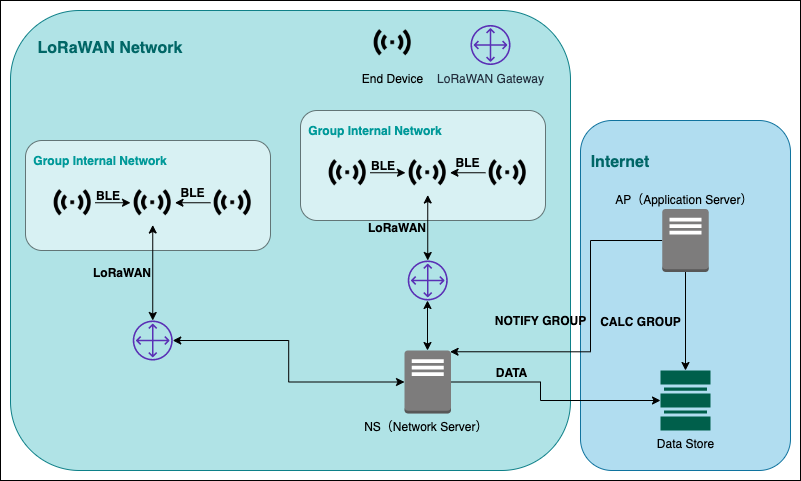
\includegraphics[width=7.5cm]{img/LoRaWAN.png}
    \caption{システム構成図}
    \label{tarako_architecture}
\end{figure}

\subsection{想定する環境}
提案方式では,隣接したセンサノード同士でグループを構成し,通信を行う.LoRaWANは,デバイスが安価であり利用において免許を必要としないため,都市部のような密集地域では,センサノードが隣接している可能性が考えられる.従って,本システムが想定する環境は,異種無線によるグループ化の適応機会が望める都市部,郊外のようなセンサノードが密集する可能性を持つ地域である.

\section{評価実験}
IoTとセンサネットワークの応用として都市におけるの情報化の推進がスマートシティとして議論されており国内の取組みも含め報告がある\cite{smart_cities}.さまざまな応用が検討されているが,都市におけるゴミ収集の効率化は社会実装が期待される応用のひとつである.例えばゴミの集積を検知するシステムの提案\cite{smart_trash_bin}や,LoRaWANを用いたセンサノードとバックエンドシステムの構築\cite{smart_waste_management}など,我々の異種無線の組み合わせによる電力効率化と補完的な研究も多いため,評価対象として都市におけるゴミ収集の効率化を取りあげる.

\subsection{実環境に基づいたシミュレーション環境の設定}
既存手法と比較し,提案手法はグループを収集したノードの情報から自動で作成するため,様々なシチュエーションにおいて展開可能である.ゴミ収集はIoTを導入したことにより,定期的な作業員の回収業務からセンサが検知した場合に回収する形態へ変化した.回収業務は効率化されるが,センサは電池給電であるためバッテリの交換作業が追加で必要となる.国内のゴミ収集におけるIoT利用例では,利用者の電源管理における負担を軽減するため,月に1度の充電で済むようシステムを提供している.電源管理のコストを削減するには,バッテリ交換時期は長く1度に交換できる数も多い方が良い.提案手法が上記の観点で,既存のLPWAソリューションと比較し有効であるか検証するため,シミュレーションを実行する.

\subsubsection{ゴミステーションにおけるグループ化}
実環境として,愛知県東浦町が発行しているゴミステーションマップ(図\ref{garbage_station_map}参照)から位置座標及びゴミ系統(燃えるゴミ・燃えないゴミ・資源ごみ)を取得し,ゴミステーションの座標をセンサの位置情報とする.各ゴミ系統に対しセンサを取り付けると仮定し,ゴミステーション毎にグループを構築する.以降,各ごみ系統に対してセンサ取り付けたものをスマートゴミ箱と称する.文献\cite{smart_garbage}を参考に,スマートゴミ箱の仕様を表\ref{tab:smart_garbage_spec}参照に示す.スマートゴミ箱の状態を超音波センサを用い3種類で把握する.

\begin{figure}[h]
    \centering
    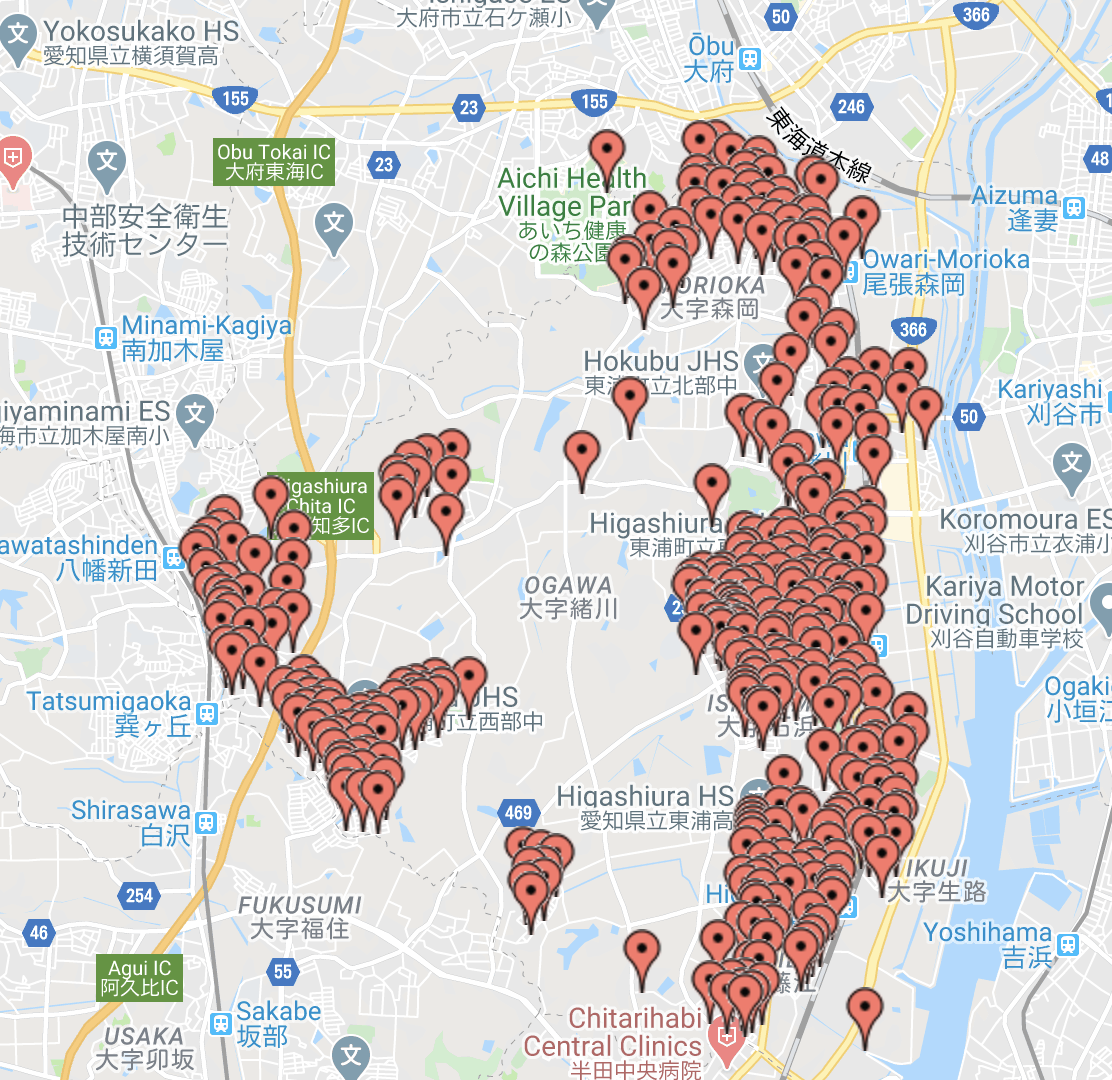
\includegraphics[width=8cm]{img/garbage_station.png}
    \caption{愛知県東浦町ゴミステーションマップ}
    \label{garbage_station_map}
\end{figure}

\begin{table}[h]
    \centering
    \caption{スマートゴミ箱の仕様}\label{tab:smart_garbage_spec}
    \begin{tabular}{|c|c|}
    \hline
    \textbf{Parameter} & \textbf{Value} \\ \hline
    status   & Empty, Filled, Full   \\ \hline
    sensor   & Ultrasonic sensor     \\ \hline
    wireless & LoRaWAN, BLE          \\ \hline
    \end{tabular}
\end{table}

\subsection{シミュレーションシナリオ}
実験の目的を達成するため以下のシミュレーションシナリオを用意した.性能評価のため,従来方式(LoRaWAN単独)と単純グループ化,平準化つきグループ化と3つのケースを試行した.ノードは,文献\cite{lorawan_usecase}より抽出した表\ref{fig:LoRaWAN_Usecase}に則り10分間に1度ゴミ箱の残容量をネットワークサーバへ送信する.表\ref{fig:group_parameter}にシミュレーションに用いたパラメーターを示す.ネットワークサーバ側で,センサデバイスとセンサデータを紐づけるため,GLのペイロードは,BLEのネットワークアドレスとセンサデータを,集約するノード分送信する.

\begin{table}[h]
    \centering
    \caption{LoRaWANのユースケース}\label{fig:LoRaWAN_Usecase}
    \scalebox{0.8}{
    \begin{tabular}{|c|c|c|c|}
    \hline
    \textbf{ケース} & \textbf{GW接続デバイス (台)} & \textbf{ゲートウェイ (台)} & \textbf{通信頻度} \\ \hline
    電灯監視        & 200               & 1                   & 1分毎           \\ \hline
    ゴミ箱          & 2000              & 4                   & 10分毎          \\ \hline
    GPSトラック     & 3000              & 5                   & 15分毎          \\ \hline
    水道メーター       & 30000             & 10                & 30分毎          \\ \hline
    パーキングメーター    & 60000             & 15              & 1時間毎          \\ \hline
    \end{tabular}
    }
\end{table}

\begin{table}[h]
    \centering
    \caption{グループ化におけるパラメータ}\label{fig:group_parameter}
    \begin{tabular}{|c|c|}
    \hline
    \textbf{Parameter}     & \textbf{Value}                \\ \hline
    number of gateways     & 1                             \\ \hline
    number of nodes        & 32                            \\ \hline
    activation time        & 0s                            \\ \hline
    connection interval    & 10m                           \\ \hline
    ble address (short)    & 4byte                         \\ \hline
    lorawan payload        & 11 \~\ 242byte                \\ \hline
    group leader payload   & 8byte * number of nodes       \\ \hline
    group member payload   & 4byte                         \\ \hline
    LoRaWAN ADR            & True                          \\ \hline
    simulation time        & 1h                            \\ \hline
    \end{tabular}
\end{table}

\subsection{消費エネルギーの計測}
消費電力量に関して,正確なエネルギーを導出することは困難であるため,消費電流量の計測をもって評価する.LoRaWANは,NS3モジュール(文献\cite{lorawan_github}参照)が提供する電力モデルを用いる.BLEは,文献\cite{ble_energy_consumption}を参考にRx(0.003A),Tx(0.003A)とする.

\subsubsection{GW・ノードの配置}
LoRaWANのGWの通信可能距離は,都市部や郊外では$5km$程度と言われている.図\ref{garbage_station_map}をもとに,全てのスマートゴミ箱に対しカバレッジを確保できるようにGWを図\ref{lorawan_area}のように配置した.シミュレーターに用いたGWの座標は表\ref{tab:gateway_position_detail}に示す.


\begin{figure}[h]
    \centering
    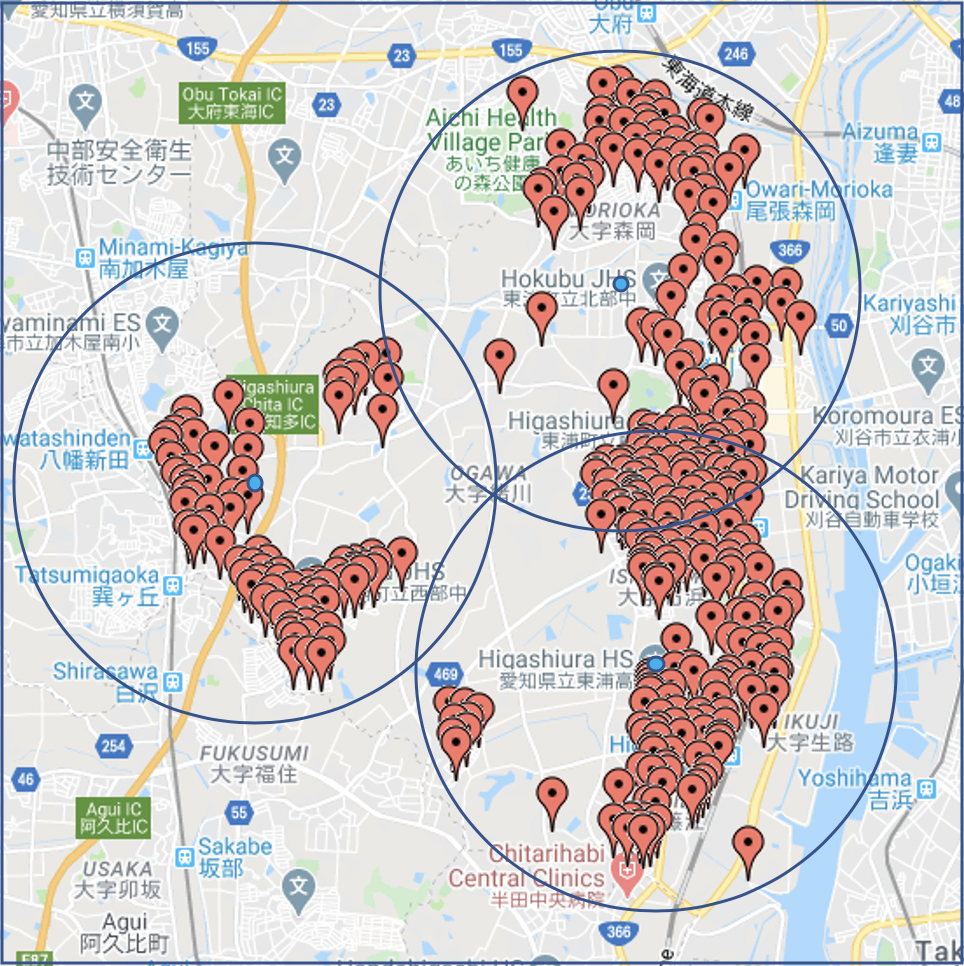
\includegraphics[width=8cm]{img/lorawan_area.png}
    \caption{カバレッジを考慮したGWの配置}
    \label{lorawan_area}
\end{figure}

\begin{table}[h]
    \centering
    \caption{ゲートウェイの配置場所詳細}
    \label{tab:gateway_position_detail}
    \begin{tabular}{|c|c|}
    \hline
    \textbf{名前}    & \textbf{座標} \\ \hline
    東浦町卯ノ里小   & (34.969392, 136.924615) \\ \hline
    愛知県立東浦高   & (34.953981, 136.962864) \\ \hline
    東浦町立北部中学校 & (34.973183, 136.967018) \\ \hline
    \end{tabular}
\end{table}

\section{結果と考察}
従来方式(LoRaWAN単独),単純グループ化,平準化つきグループ化について,ノード毎の消費電流量をまとめた.シミュレーターの都合上,町内全てのノードでの再現が難しかったため地域を限定し行った.対象地域では,全てのグループが3ノードで構成されている.LoRaWANノードに割り当てるデータレートをADRにて自動で調節し全てのケースでDR5を選択したまた,消費電流量の値を元にバッテリー交換機会についての言及も行う.バッテリーの参考値として,屋外でのLoRaWANモジュール\cite{outdoor_lorawan_module}に搭載されている充電式バッテリー(4100mAh)を用いる.シミュレーターでの実測値と実際の製品のスペックとの間に差があったため,前者に合わせBLEの負荷電流を調整しシミューションを行った.計測した各通信方式の1送信あたりの消費電流量を表\ref{one_shot_cc}に示す.

\begin{table}[h]
    \centering
    \caption{1送信あたりの消費電流量(グループは3ノードの場合)}
    \label{tab:one_shot_cc}
    \begin{tabular}{|c|c|}
    \hline
    \textbf{Parameter} & \textbf{Value}   \\ \hline
    LoRaWAN                   & 8mA       \\ \hline
    GL(単純グループ化)         & 13.4mA    \\ \hline
    GM(単純グループ化)         & 0.6mA     \\ \hline
    GL(平準化つきグループ化)    & 14.4mA    \\ \hline
    GM(平準化つきグループ化)    & 1.2mA     \\ \hline
    \end{tabular}
\end{table}

\subsection{従来方式(LoRaWAN単独)}
1時間あたりの従来方式(LoRaWAN単独)の消費電流量を図\ref{energy_consumption_only_lorawan}に示す.その他取得した値を表\ref{tab:lorawan_result}に示す.いずれのノードも消費電流量は均一で,差分は0.001A(≒1mA)とLoRaWAN1送信分にも満たない小さい値であった.ノード間で差が起きた理由としては,図\ref{garbage_box_diss_location}より,スマートゴミ箱が設置されている箇所によりGWとの距離に差があるためである.バッテリー交換機会に関して,表\ref{tab:one_shot_cc}の値を用いてバッテリーの持ち時間を計算すると,10分に1度の送信というユースケースで約21日間利用可能である.ノードのバッテリー残量が均一に減少するため,スマートゴミ箱のグループ単位で交換作業を同時に行うことが可能である.

\begin{figure}[h]
    \centering
    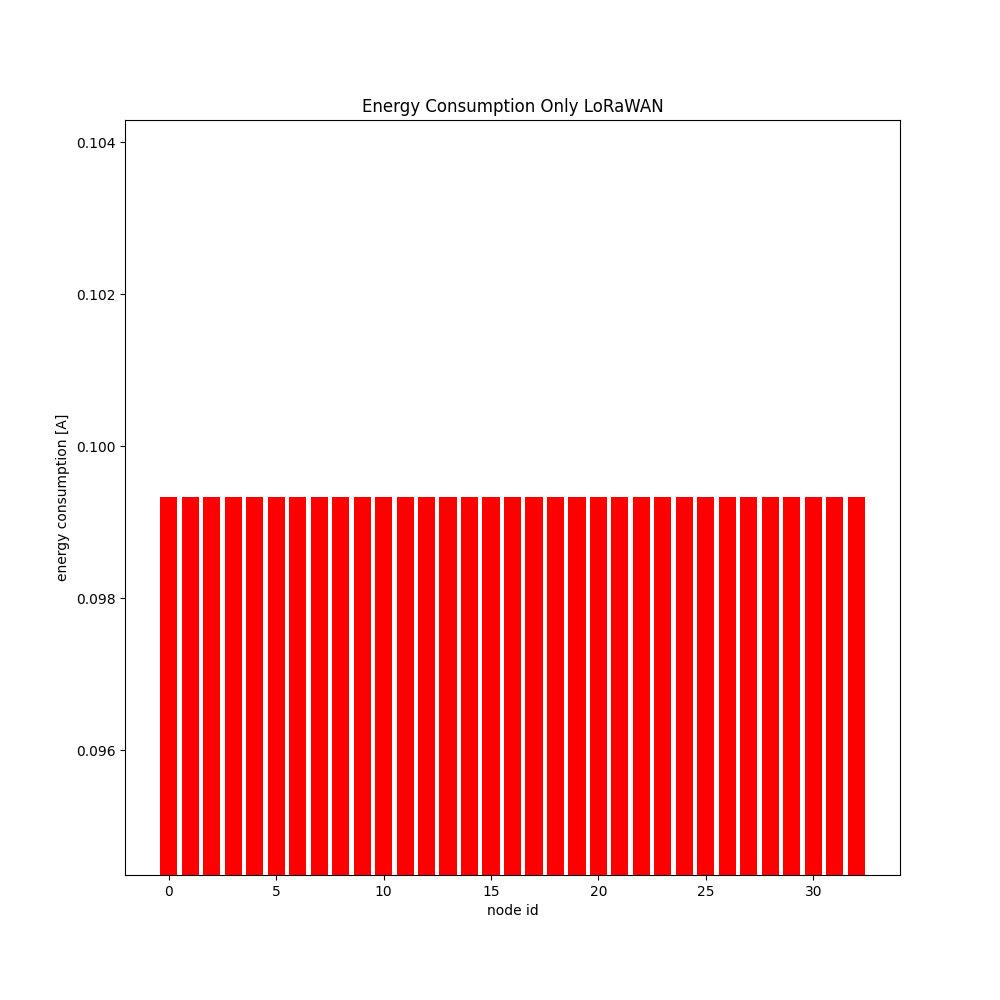
\includegraphics[width=8cm]{img/lorawan_energy_consumption.png}
    \caption{従来方式(LoRaWAN単独)の消費電流量}
    \label{energy_consumption_only_lorawan}
\end{figure}

\begin{table}[h]
    \centering
    \caption{従来方式(LoRaWAN単独)の結果}
    \label{tab:lorawan_result}
    \begin{tabular}{|c|c|}
    \hline
    \textbf{Parameter} & \textbf{Value}   \\ \hline
    ネットワーク全体の消費電流量              & 1.627A     \\ \hline
    パケット到達率(LoRaWaN)               & 100\%\     \\ \hline
    ノード間の消費電流量における差分最大値      & 0.001A     \\ \hline
    \end{tabular}
\end{table}

\begin{figure}[h]
    \centering
    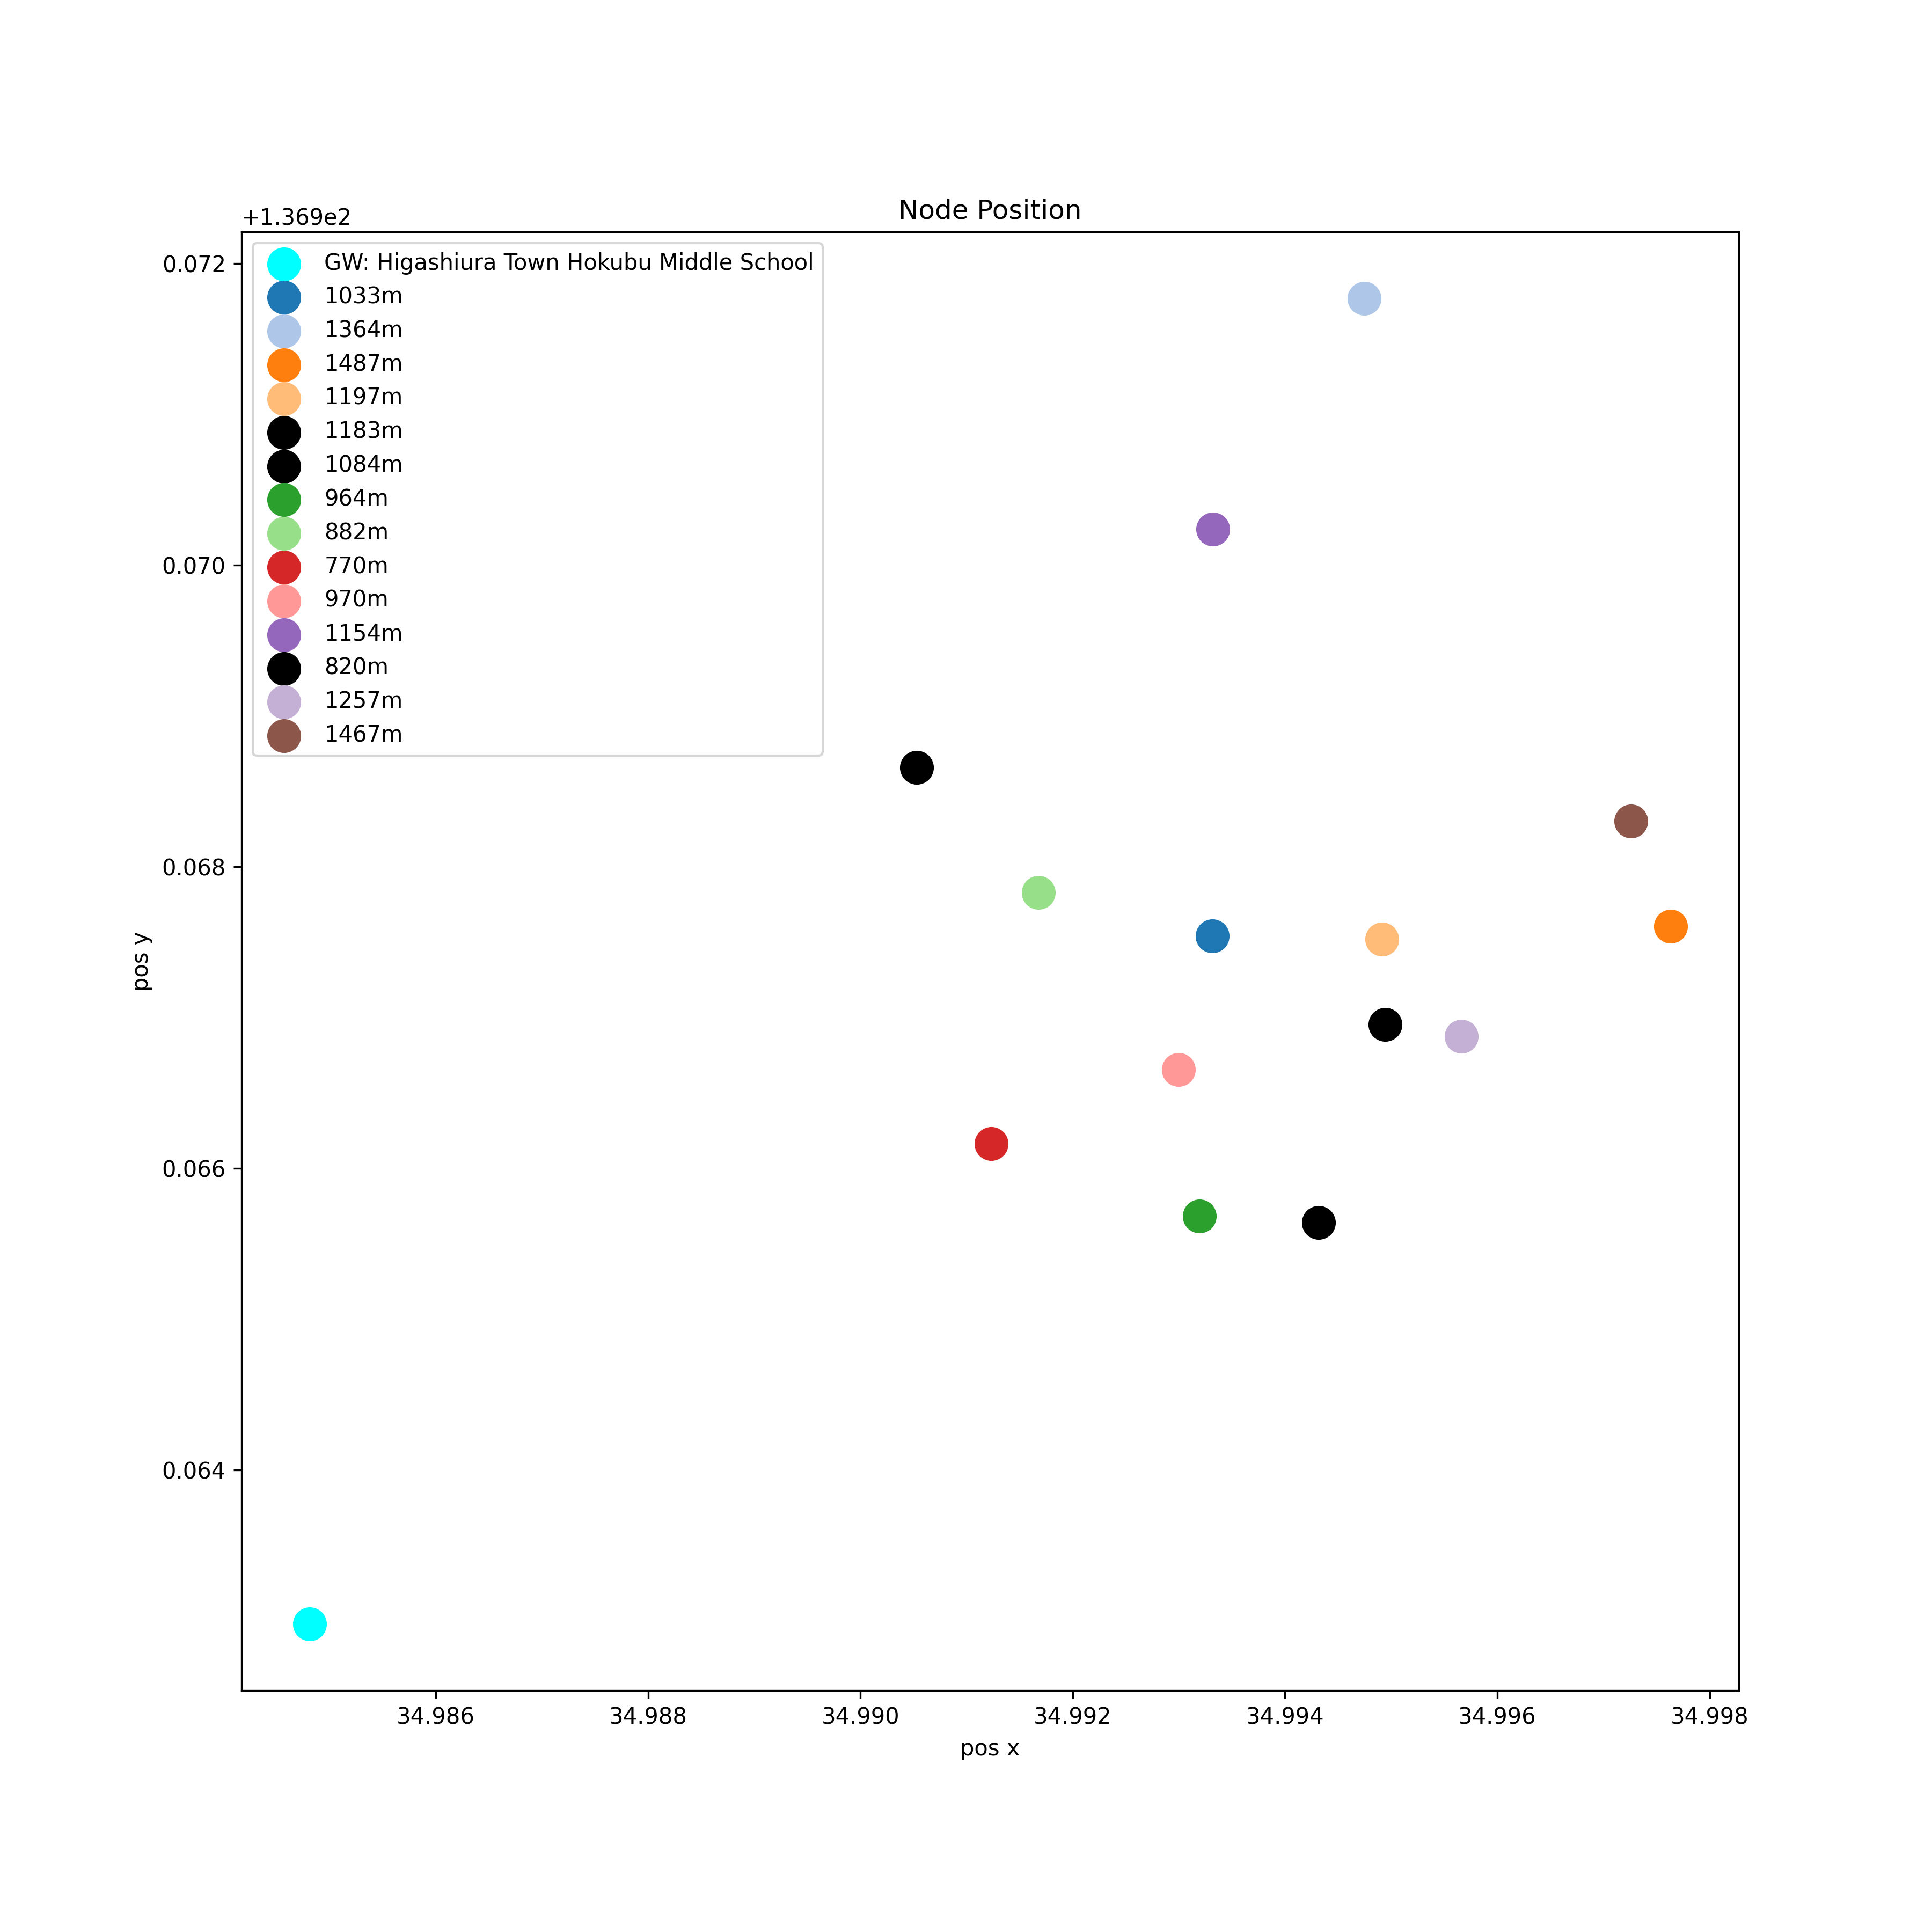
\includegraphics[width=8cm]{img/garbage_box_location.png}
    \caption{GWと各ノードの距離関係}
    \label{garbage_box_diss_location}
\end{figure}

\subsection{単純グループ化}
1時間あたりのグループ化の消費電流量を図\ref{energy_consumption_grouping_without_eq}に示す.1時間毎の消費電流量を図\ref{gec_all}に示す.その他取得した値を表\ref{tab:simple_grouping_result}に示す.棒グラフの配色について,黒は設置されているスマートゴミ箱が単体であるため,構築できるグループが存在しないという理由からLoRaWANのみを用いて通信するノード,その他は参加するグループ毎に割り当てられている.図\ref{energy_consumption_grouping_without_eq}を見ると,GLノードに消費電流量が偏っている.表\ref{tab:one_shot_cc}より,従来方式(LoRaWAN単独)と比較しGLノードの消費電流量に差が生じたのは,GMノードのセンサデータを集約した分,送信データ量が増加したことによる割り当てられる通信時間の増加であると考えられる.表\ref{tab:simple_grouping_result}より,パケット到達率はいずれの通信方式においても100 \%\ を示した.バッテリー交換機会に関して,表\ref{tab:one_shot_cc}の値を用いてバッテリーの持ち時間を計算すると,前述したユースケースで,GLノードが約13日,GMノードが約285日間利用可能である.

\begin{figure}[h]
    \centering
    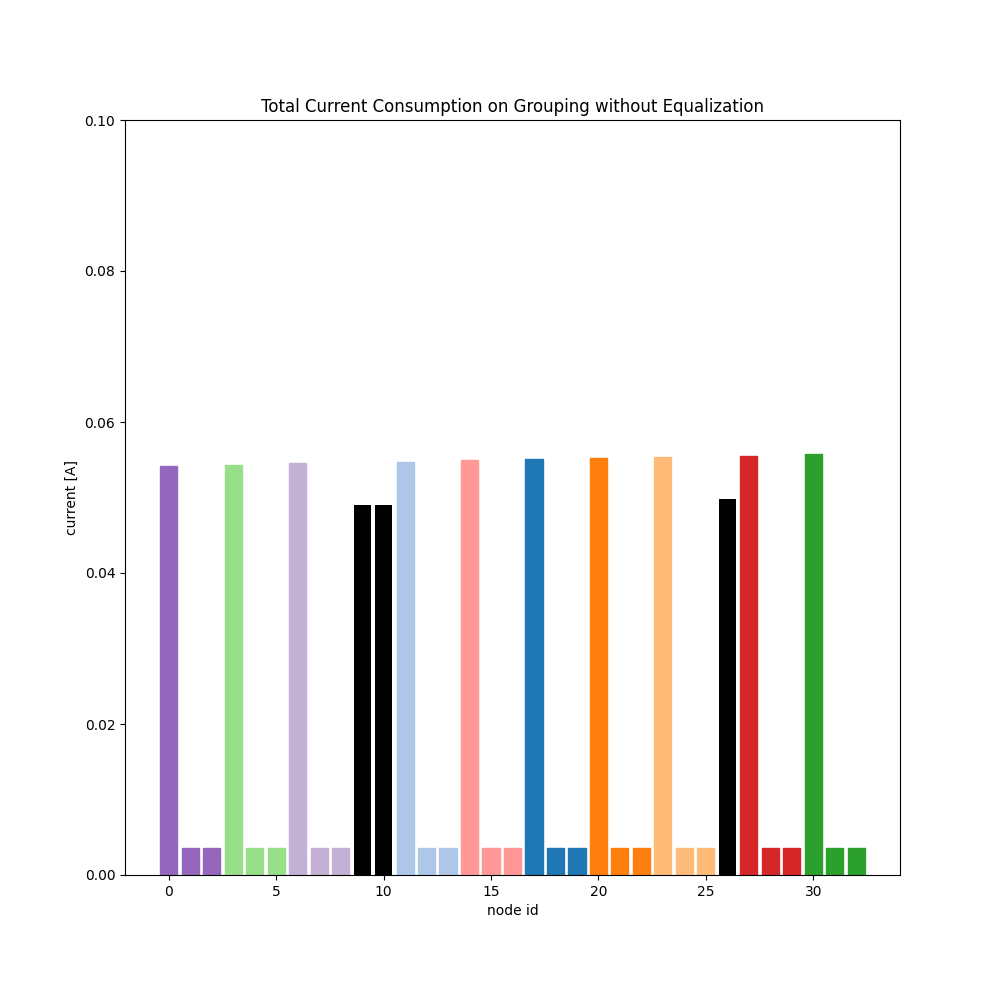
\includegraphics[width=8cm]{img/group_without_eq/group_consumption_without_eq_1_hour.png}
    \caption{単純グループ化の消費電流量(LoRaWAN単独比較用)}
    \label{energy_consumption_grouping_without_eq}
\end{figure}

\begin{figure}[h]
    \centering
    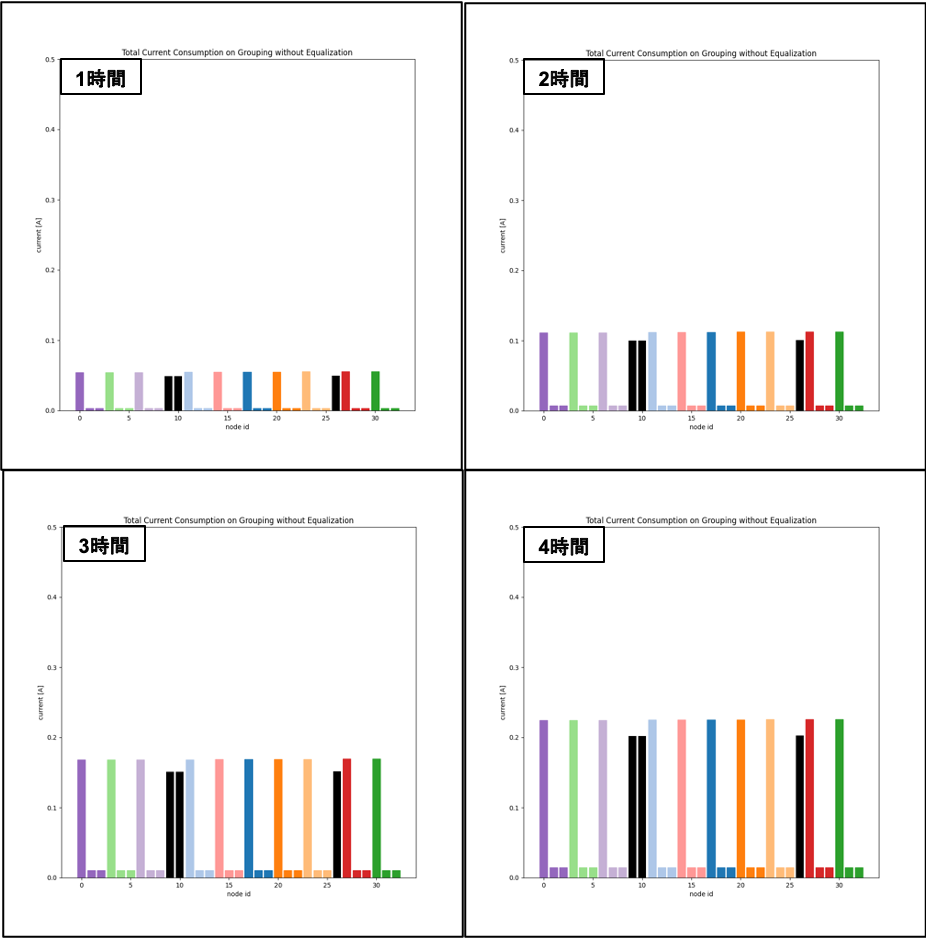
\includegraphics[width=7.5cm]{img/group_without_eq/all.png}
    \caption{単純グループ化の消費電流量}
    \label{gec_all}
\end{figure}

\begin{table}[h]
    \centering
    \caption{単純グループ化の消費電流量まとめ}
    \label{tab:simple_grouping_result}
    \scalebox{0.8}[0.8]{
    \begin{tabular}{|c|c|c|c|c|}
    \hline
    \textbf{時間} & \
    \begin{tabular}{c} \textbf{ネットワーク全体の} \\ \textbf{消費電流量} \end{tabular} & \
    \begin{tabular}{c} \textbf{ノード間の} \\ \textbf{消費電流量における} \\ \textbf{差分最大値} \end{tabular} \\ \hline
    1時間 & 0.769A & 0.052A \\ \hline
    2時間 & 1.565A & 0.106A \\ \hline
    3時間 & 2.356A & 0.158A \\ \hline
    4時間 & 3.147A & 0.212A \\ \hline
    \end{tabular}
    }
\end{table}

\begin{table}[h]
    \centering
    \caption{単純グループ化のパケット到達率}
    \label{tab:simple_grouping_result}
    \scalebox{0.8}[0.8]{
    \begin{tabular}{|c|c|c|c|c|}
    \hline
    \textbf{時間} & \
    \begin{tabular}{c} \textbf{パケット到達率}   \\ \textbf{(LoRaWaN)} \end{tabular} & \
    \begin{tabular}{c} \textbf{パケット到達率}   \\ \textbf{(BLE)} \end{tabular} \\ \hline
    1時間 & 100 \%\  & 100 \%\ \\ \hline
    2時間 & 100 \%\  & 100 \%\ \\ \hline
    3時間 & 100 \%\  & 100 \%\ \\ \hline
    4時間 & 100 \%\  & 100 \%\ \\ \hline
    \end{tabular}
    }
\end{table}

\subsection{平準化つきグループ化}
GLノードの交換頻度が毎回であるケースの1時間毎の消費電流量を,図\ref{with_eq_1time}に示す.表\ref{gec_with_eq_1time_all}を元に,前述した単純グループ化と比較すると,ノード間の消費電流量の差分が,0.052Aから0.026Aと半分に削減された.これは,GLノードが送信するごとに次のGLノードを選出し切り替えを行ったためである.図\ref{gec_with_eq_1time_all},表\ref{tab:one_shot_cc}を見ると,従来方式(LoRaWAN単独)と比較し,平準化つきグループ化ではデータを集約すること,GLノード通知のためBLEによる通信回数が増えることの2つの理由から,バッテリー交換のタイミングを合わせようとすると消費電流量が増加する傾向にある.

\begin{figure}[h]
    \centering
    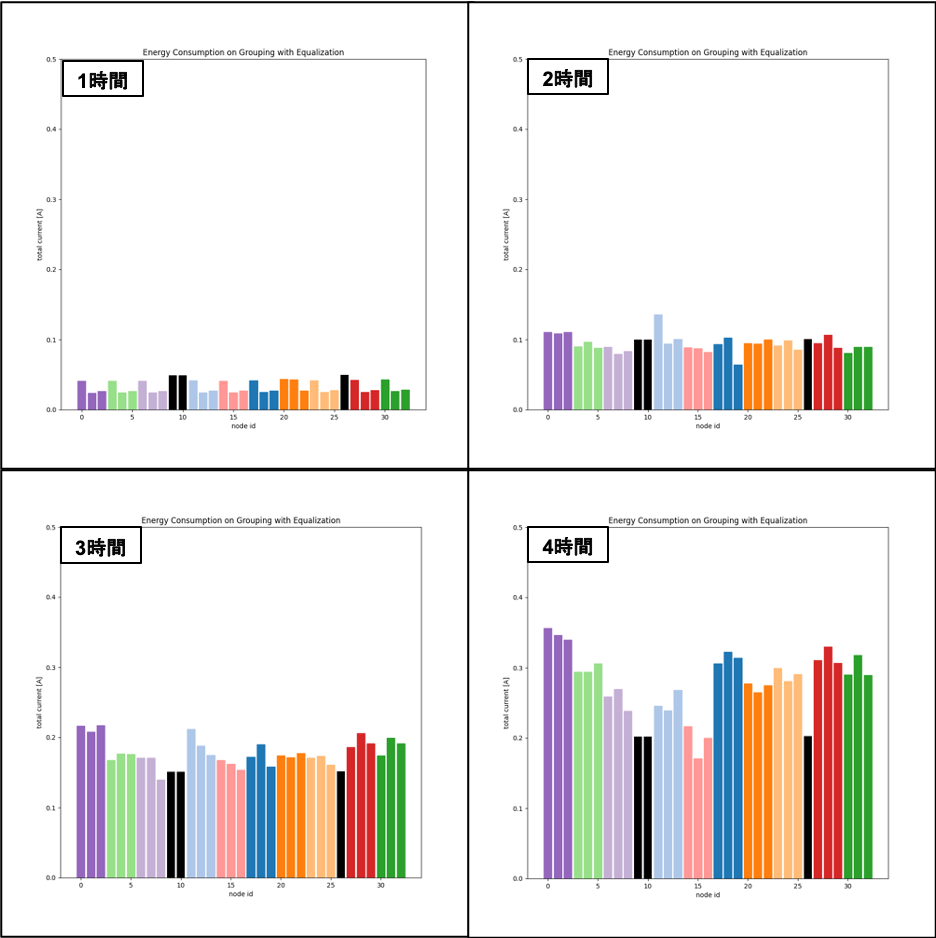
\includegraphics[width=7.5cm]{img/group_with_eq/1time.png}
    \caption{平準化つきグループ化の消費電流量(交替頻度:毎回)}
    \label{with_eq_1time}
\end{figure}

\begin{table}[h]
    \centering
    \caption{平準化つきグループ化の消費電流量まとめ(交替頻度:毎回)}
    \label{tab:with_eq_1time_ec}
    \scalebox{0.8}[0.8]{
    \begin{tabular}{|c|c|c|}
    \hline
    \textbf{時間} & \
    \begin{tabular}{c} \textbf{ネットワーク全体の} \\ \textbf{消費電流量} \end{tabular} & \
    \begin{tabular}{c} \textbf{ノード間の} \\ \textbf{消費電流量における} \\ \textbf{差分最大値} \end{tabular} \\ \hline
    1時間 & 1.105A & 0.026A \\ \hline
    2時間 & 3.121A & 0.072A \\ \hline
    3時間 & 5.852A & 0.077A \\ \hline
    4時間 & 9.126A & 0.185A \\ \hline
    \end{tabular}
    }
\end{table}

\begin{table}[h]
    \centering
    \caption{平準化つきグループ化のパケット到達率(交替頻度:毎回)}
    \label{tab:with_eq_1time_packet}
    \scalebox{0.8}[0.8]{
    \begin{tabular}{|c|c|c|c|c|}
    \hline
    \textbf{時間} & \
    \begin{tabular}{c} \textbf{パケット到達率}   \\ \textbf{(LoRaWaN)} \end{tabular} & \
    \begin{tabular}{c} \textbf{パケット到達率}   \\ \textbf{(BLE)} \end{tabular} \\ \hline
    1時間 & 100 \%\   & 86 \%\ \\ \hline
    2時間 & 99  \%\   & 82 \%\ \\ \hline
    3時間 & 96  \%\   & 78 \%\ \\ \hline
    4時間 & 96  \%\   & 73 \%\ \\ \hline
    \end{tabular}
    }
\end{table}

\subsubsection{GLノードの交換タイミングによる比較}
グループ内での通信回数を減らし,消費電力を削減するためGLノードの交替頻度を変更しシミュレーションを実行した.グループ内の集約回数が2回でGLノードを更新する場合の結果を,図\ref{with_eq_2time},表\ref{tab:with_eq_2time_ec},表\ref{tab:with_eq_2time_packet}に示す.グループ内の集約回数が3回でGLノードを更新する場合の結果を,図\ref{with_eq_3time},表\ref{tab:with_eq_3time_ec},表\ref{tab:with_eq_3time_packet}に示す.図\ref{with_eq_2time},図\ref{with_eq_3time}を見ると,交換頻度が低くなるほどLoRaWAN単独でのノードとの消費電流量差が小さくなっている.交換頻度が3回に1回になった際に,グループを構築しているノード方が消費電流量を下回り始めた.これは,表\ref{tab:simple_grouping_result}より,GLノード切り替えを行わない方式の場合はパケット到達率が100 \%\ であること,表\ref{tab:with_eq_1time_packet},表\ref{tab:with_eq_2time_packet},表\ref{tab:with_eq_3time_packet}より,原因としてGLノードのダウンリンクが増えたことからBLEでのパケット到達率が減少し,GLノードの切り替えが上手くいっていない事が考えられる.また,GLノードの交換頻度の間隔が長くなり,時間が経過するとともにパケット到達率が減少していることから,通信タイミングの制御を考慮する必要がある.

\begin{figure}[h]
    \centering
    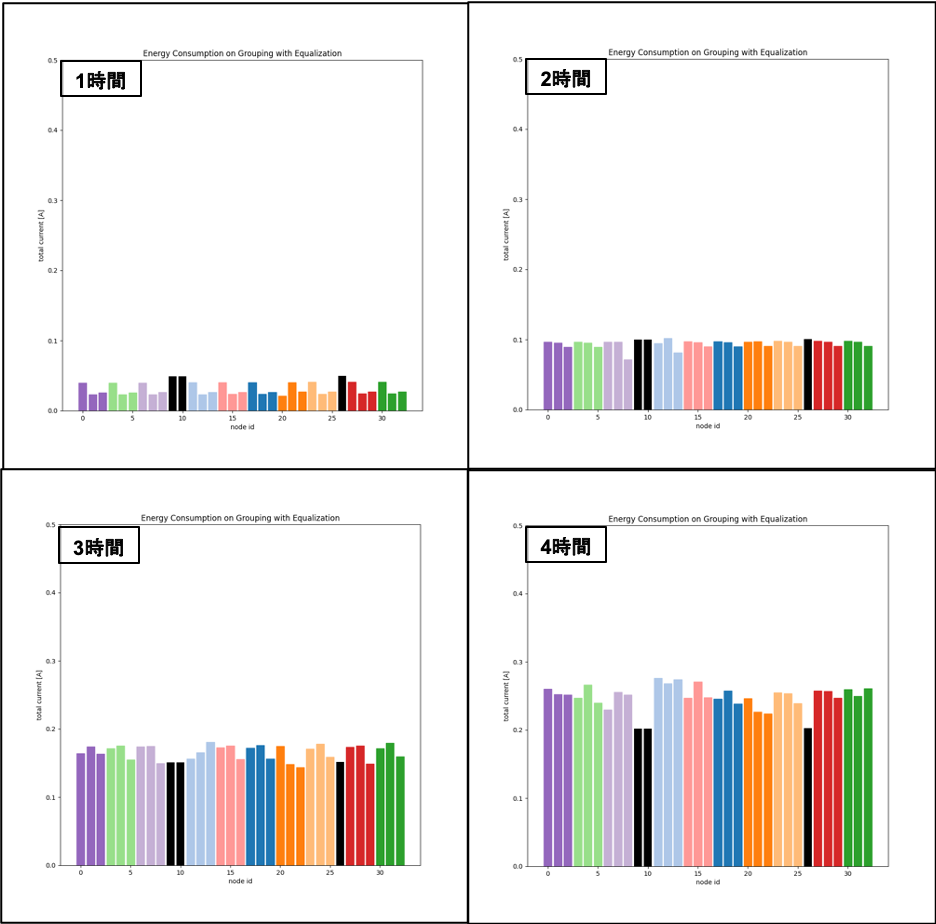
\includegraphics[width=7.5cm]{img/group_with_eq/2time.png}
    \caption{平準化つきグループ化の消費電流量まとめ(交替頻度:送信2回に1回)}
    \label{with_eq_2time}
\end{figure}

\begin{table}[h]
    \centering
    \caption{平準化つきグループ化の消費電流量まとめ(交替頻度:送信2回に1回)}
    \label{tab:with_eq_2time_ec}
    \scalebox{0.8}[0.8]{
    \begin{tabular}{|c|c|c|c|c|}
    \hline
    \textbf{時間} & \
    \begin{tabular}{c} \textbf{ネットワーク全体の} \\ \textbf{消費電流量} \end{tabular} & \
    \begin{tabular}{c} \textbf{ノード間の} \\ \textbf{消費電流量における} \\ \textbf{差分最大値} \end{tabular} \\ \hline
    1時間 & 1.052A & 0.029A \\ \hline
    2時間 & 3.116A & 0.030A  \\ \hline
    3時間 & 5.452A & 0.037A \\ \hline
    4時間 & 8.163A & 0.074A \\ \hline
    \end{tabular}
    }
\end{table}

\begin{table}[h]
    \centering
    \caption{平準化つきグループ化のパケット到達率(交替頻度:送信2回に1回)}
    \label{tab:with_eq_2time_packet}
    \scalebox{0.8}[0.8]{
    \begin{tabular}{|c|c|c|c|c|}
    \hline
    \textbf{時間} & \
    \begin{tabular}{c} \textbf{パケット到達率}   \\ \textbf{(LoRaWaN)} \end{tabular} & \
    \begin{tabular}{c} \textbf{パケット到達率}   \\ \textbf{(BLE)} \end{tabular} \\ \hline
    1時間 & 100\%\   & 80 \%\ \\ \hline
    2時間 & 99 \%\   & 86 \%\ \\ \hline
    3時間 & 96 \%\   & 80 \%\ \\ \hline
    4時間 & 92 \%\   & 75 \%\ \\ \hline
    \end{tabular}
    }
\end{table}


\begin{figure}[h]
    \centering
    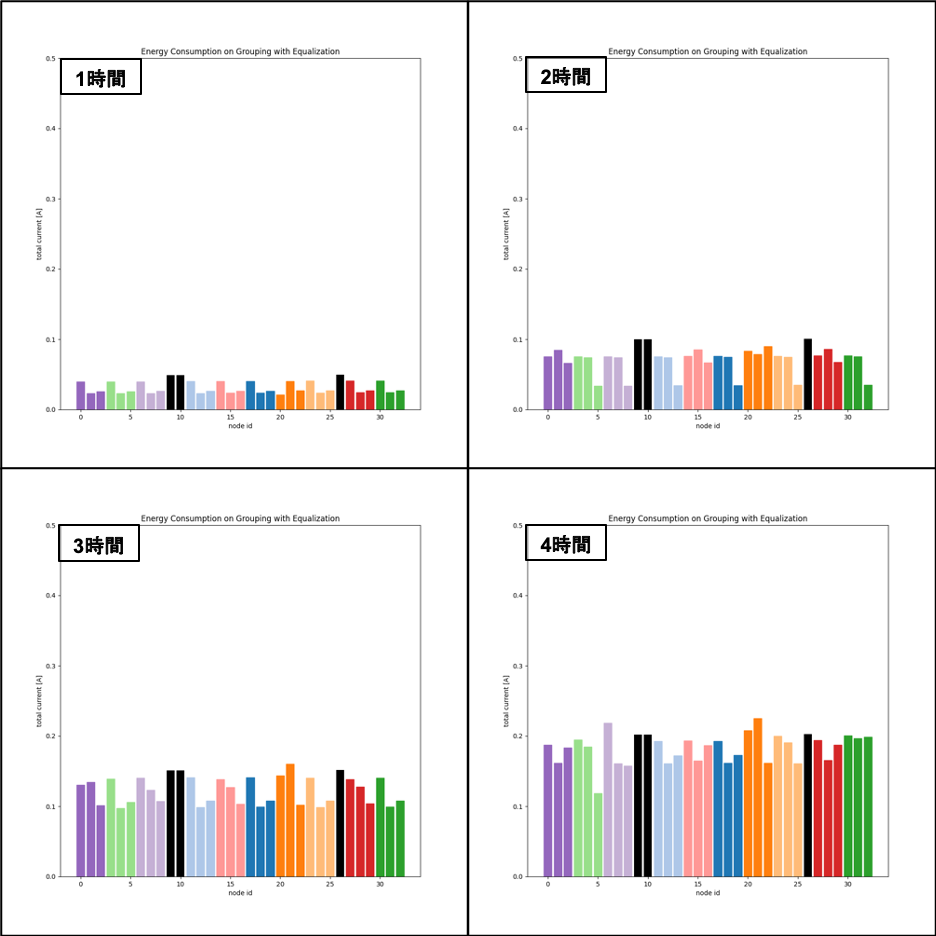
\includegraphics[width=7.5cm]{img/group_with_eq/3time.png}
    \caption{平準化つきグループ化の消費電流量(交替頻度:送信3回に1回)}
    \label{with_eq_3time}
\end{figure}

\begin{table}[h]
    \centering
    \caption{平準化つきグループ化の消費電流量まとめ(交替頻度:送信3回に1回)}
    \label{tab:with_eq_3time_ec}
    \scalebox{0.8}[0.8]{
    \begin{tabular}{|c|c|c|c|c|}
    \hline
    \textbf{時間} & \
    \begin{tabular}{c} \textbf{ネットワーク全体の} \\ \textbf{消費電流量} \end{tabular} & \
    \begin{tabular}{c} \textbf{ノード間の} \\ \textbf{消費電流量における} \\ \textbf{差分最大値} \end{tabular} \\ \hline
    1時間 & 1.052A & 0.029A  \\ \hline
    2時間 & 2.347A & 0.067A  \\ \hline
    3時間 & 4.07A  & 0.063A  \\ \hline
    4時間 & 6.061A & 0.107A  \\ \hline
    \end{tabular}
    }
\end{table}

\begin{table}[h]
    \centering
    \caption{平準化つきグループ化のパケット到達率(交替頻度:送信3回に1回)}
    \label{tab:with_eq_3time_packet}
    \scalebox{0.8}[0.8]{
    \begin{tabular}{|c|c|c|c|c|}
    \hline
    \textbf{時間} & \
    \begin{tabular}{c} \textbf{パケット到達率}   \\ \textbf{(LoRaWaN)} \end{tabular} & \
    \begin{tabular}{c} \textbf{パケット到達率}   \\ \textbf{(BLE)} \end{tabular} \\ \hline
    1時間 & 100 \%\ & 80 \%\ \\ \hline
    2時間 & 99 \%\  & 71 \%\ \\ \hline
    3時間 & 99 \%\  & 69 \%\ \\ \hline
    4時間 & 93 \%\  & 71 \%\ \\ \hline
    \end{tabular}
    }
\end{table}

\section{おわりに}
WSNでは,電池駆動型のIoTセンサでは省電力化の議論がされている.WSNの中でも,LoRaWANという長距離通信,低消費電力を特徴とする通信規格では都市部や市街地のような密集地において,ノードの台数が増加した際に,通信の衝突から再送が発生し結果としてバッテリー寿命が短命化するという課題がある.そこで我々は,WSNの消費電力効率化(消費電力削減・消費電力平準化)のためのBLE,LoRaを組み合わせた異種無線によるノードのグループ化の実現を本研究の目的においた.目的の実現のために,既存の通信規格のプロトコルを変更せず異種無線の消費電力効率化が実現可能なシステムを設計した.提案したシステムは,ノードが収集可能な情報からのグループ構築機能,各ノードの通信における,Rx,Txの理論値及び通信利用回数等からバッテリー残量を算出し,GLの切り替えを行う電力平準化機能を実装することで,WSNのオペレーターは,既存の通信方式と同様の利用で,バッテリー寿命を延伸することが実現可能となる.
\par
その有効性を確認するため,提案システムをごみ収集のスマートIoT化を話題とし,実世界を再現しシミュレーションを行った.
\par
平準化つきグループ化において,パケット到達率向上のためGLノードのダウンリンクのタイミングを調整するという課題が挙げられる.今後はグループ内でBLEの通信が衝突しない手法を検討する予定である.

\begin{thebibliography}{4}
    \bibitem{me_research} 戸澤涼, 稲村浩, 中村嘉隆:  高集積センサネットワークにおける異種無線を用いた電力効率化の研究, 情報処理, Vol.82, No.3, pp.97-98 (2020)
    
    \bibitem{garbage_station} オープンデータ ごみステーション|東浦町(最終閲覧日:2020年3月10日), \url{https://www.town.aichi-higashiura.lg.jp/soshiki/kohojoho/kohotokei/gyomu/opendata/1514185444468.html}

    \bibitem{gateway} 辻丸勇樹, 坂本龍一, 近藤正章, 中村宏: LPWA通信を利用するIoTプラットフォーム向けの電力効率を考慮したゲートウェイ配置手法の検討, 情報処理学会研究報告会, Vol.32, No.1, pp.46–53(2017)

    \bibitem{group} 手柴瑞基, 湯素華, 小花貞夫: LoRaWANにおけるネットワーク効率化のためのノードのグループ構成法と通信制御方式, 情報処理学会研究報告会, Vol.89, No.13, pp.1-8(2018)

    \bibitem{lora_signal_coverage} Dambal, Vageesh and Mohadikar, Sameer and Kumbhar, Abhaykumar and Guvenc, Ismail: Improving LoRa Signal Coverage in Urban and Sub-Urban Environments with UAVs, arXiv, 1902.11243(2019)

    \bibitem{lorawan_energy_efficiency} Wu, He and Nabar, Sidharth and Poovendran, Radha: An Energy Framework for the Network Simulator 3 (ns-3), SIMUTools 2011 - 4th International ICST Conference on Simulation Tools and Techniques, 

    \bibitem{lorawan_range} LoRaWAN Range Part 2: Range and Coverage of LoRaWAN in Practice (Updated)(最終閲覧日:2020年4月6日), \url{https://smartmakers.io/en/lorawan-range-part-2-range-and-coverage-of-lorawan-in-practice}

    \bibitem{lorawan_github} signetlabdei/lorawan: \url{https://github.com/signetlabdei/lorawan}

    \bibitem{smart_garbage} Joni, Koko and Haryanto, Haryanto and Rohim, D: Smart Garbage Based on Internet of Things (IoT), Journal of Physics: Conference Series, Vol.953, pp.012189

    \bibitem{lorawan_usecase} 1台のLoRaゲートウェイでどれくらいのデバイスに対応できますか?(最終閲覧日:2020年4月30日), \url{https://soracom.zendesk.com/hc/ja/articles/115001237211-%EF%BC%91%E5%8F%B0%E3%81%AELoRa%E3%82%B2%E3%83%BC%E3%83%88%E3%82%A6%E3%82%A7%E3%82%A4%E3%81%A7%E3%81%A9%E3%82%8C%E3%81%8F%E3%82%89%E3%81%84%E3%81%AE%E3%83%87%E3%83%90%E3%82%A4%E3%82%B9%E3%81%AB%E5%AF%BE%E5%BF%9C%E3%81%A7%E3%81%8D%E3%81%BE%E3%81%99%E3%81%8B-}

    \bibitem{ble_energy_consumption} Power consumption analysis of bluetooth low energy commercial products and theirimplications for IoT applications.Electronics (Switzerland), 7(12), 2018

    \bibitem{smart_cities} Khatoun, Rida and Zeadally, Sherali: Smart cities: concepts, architectures, research opportunities, Communications of the ACM, Vol.59, No.8, 2016

    \bibitem{smart_trash_bin} Kristanto, Slamet and Yashiro, Takeshi and Koshizuka, Noboru and Sakamura, Ken: Dynamic Polling Algorithm for Low Energy Garbage Level Measurement in Smart Trash Bin, Proceedings of the Second International Conference on IoT in Urban Space, No.92-94, 2016

    \bibitem{smart_waste_management} Fedchenkov, Petr and Zaslavsky, Arkady and Sosunova, Inna: Enabling Smart Waste Management with Sensorized Garbage Bins and Low Power Data Communications Network, Proceedings of the Seventh International Conference on the Internet of Things, No.28, 2017

    \bibitem{outdoor_lorawan_module} Outdoor LoRa/LoRaWAN Wireless I/O Module(最終閲覧日:2020年5月7日), \url{https://www.advantech.com/products/23ed4776-1633-4901-a776-8532a23ea8b4/wise-4610/mod_b9c0a2e0-c841-4826-8008-36a91d837e1e}

\end{thebibliography}

\end{document}
